\documentclass[10.5pt]{config}
% 本实验报告采用 署名-相同方式共享 4.0 国际许可协议 (CC BY-SA 4.0)
\usepackage{bigstrut,multirow,rotating,booktabs,makecell,array}%表格插件

\major{电子科学与技术}
\name{郑智瑄}
\partner{} % 签名栏
% \title{}
\stuid{3230103913}
\date{\today}
\lab{东4-421}
\course{电子工程训练（甲）}
\instructor{马洪庆}
\grades{}
\expname{电子工训基础部分} % 实验名字
\exptype{测试型} % 实验类型

\begin{document}

% \maketitlepage % 封面
% \maketoc % 目录
\makeheader % 首页头部


\section{电子仪器的使用练习}
\subsection{万用表的使用练习（测量前需将万用表打到合适的档位）：}
\subsubsection{取三个不同色环的电阻，读取电阻标称值、允许偏差，用万用表测量其阻值并记
录，计算电阻偏差（设计合适的表格用于记录读取值、测量值及计算值。偏差指相对偏差，
用\%表示，下同）}

\begin{table}[H]
    \centering
    \caption{电阻测量数据}
    \begin{tabular}{|>{\centering\arraybackslash}c|>{\centering\arraybackslash}c|>{\centering\arraybackslash}c|>{\centering\arraybackslash}c|>{\centering\arraybackslash}c|>{\centering\arraybackslash}c|>{\centering\arraybackslash}c|>{\centering\arraybackslash}c|>{\centering\arraybackslash}c|}
    \hline
    \multirow{2}[4]{*}{组别} & \multirow{2}[4]{*}{色环颜色} & \multirow{2}[4]{*}{标称值} & \multirow{2}[4]{*}{允许偏差} & \multicolumn{4}{c|}{测量值} & \multirow{2}[4]{*}{实际误差} \bigstrut\\
    \cline{5-8}
          &       &       &       & 第1次   & 第2次   & 第3次   & 平均值   &  \bigstrut\\
    \hline
    1     & 棕黑黑黄棕 & $1M\Omega$    & 1\%   & $1.0033M\Omega$  & $1.003M\Omega$  & $1.0036M\Omega$  & $1.0033M\Omega$  & 0.33\% \bigstrut\\
    \hline
    2     & 黄紫黑橙棕 & $0.47M\Omega$  & 1\%   & $0.4871M\Omega$  & $0.4873M\Omega$  & $0.4868M\Omega$  & $0.4871M\Omega$  & 3.63\% \bigstrut\\
    \hline
    3     & 橙黑黑橙棕 & $0.3M\Omega$   & 1\%   & $0.2993M\Omega$  & $0.2996M\Omega$  & $0.2995M\Omega$  & $0.2995M\Omega$  & -0.18\% \bigstrut\\
    \hline
    \end{tabular}%
    \label{tab:addlabel}%
\end{table}%

【数据分析】：1与3满足允许偏差，测量准确；2超出了允许偏差，可能是电阻制作超过了允差

\subsubsection{取三个不同电容值的电容，读取电容的标称值，用万用表测量其电容并记录，计
算电容偏差。}

% Table generated by Excel2LaTeX from sheet 'Sheet1'
\begin{table}[H]
  \centering
  \caption{电容测量数据}
    \begin{tabular}{|c|c|>{\centering\arraybackslash}c|c|c|c|c|}
    \hline
    \multirow{2}[4]{*}{组别} & \multirow{2}[4]{*}{标称值} & \multicolumn{4}{c|}{测量值} & \multirow{2}[4]{*}{实际误差} \bigstrut\\
\cline{3-6}          &       & 第1次   & 第2次   & 第3次   & 平均值   &  \bigstrut\\
  \hline
  1     & $1\mu F$   & $1.0894\mu F$ & $1.0955\mu F$ & $1.0924\mu F$ & $1.0924\mu F$ & 9.24\% \bigstrut\\
  \hline
  2     & $47\mu F$  & $59.50\mu F$ & $59.37\mu F$ & $59.56\mu F$ & $59.48\mu F$ & 26.55\% \bigstrut\\
  \hline
  3     & 1nF   & 0.99nF & 0.979nF & 0.980nF & 0.983nF & -1.70\% \bigstrut\\
  \hline
    \end{tabular}%
  \label{tab:addlabel}%
\end{table}%

【数据分析】：相较于电阻，电容的实际误差要大很多，猜测可能是由于电容测量由于充放电特殊性较难测量，且频率敏感，受环境影响大。同时，对于 $47\mu F$电容，经多次测量，且等待直至示数稳定所得数值均偏大，询问老师得知大电容偏差较大正常。


\subsubsection{取一个二极管，用万用表判断其极性，测量它的正向导通压降，并记录。（将万用
表打到“二极管测量/蜂鸣”档位，按下万用表面板上的“SELECT”按钮，选择“二极管测
量”）。}

\begin{table}[H]
  \centering
  \caption{二极管导通压降数据}
    \begin{tabular}{|c|c|c|c|}
    \hline
    \multicolumn{4}{|c|}{测量值} \bigstrut\\
    \hline
    第1次   & 第2次   & 第3次   & 平均值 \bigstrut\\
    \hline
    0.6447V & 0.6445V & 0.6442V & 0.6445V \bigstrut\\
    \hline
    \end{tabular}%
  \label{tab:addlabel}%
\end{table}%

\subsubsection{取一个三极管，用万用表确定它的集电极、基级和发射极，画出三极管外观图并
标注管脚。（将万用表打到hFE档测试，如果测量正确，屏幕上会有相应的hFE数值显示）。}

\begin{table}[H]
  \centering
  \caption{hFE数值}
    \begin{tabular}{|c|c|c|c|}
    \hline
    \multicolumn{4}{|c|}{测量值} \bigstrut\\
    \hline
    第1次   & 第2次   & 第3次   & 平均值 \bigstrut\\
    \hline
    371   & 374   & 373   & 372.67 \bigstrut\\
    \hline
    \end{tabular}%
  \label{tab:addlabel}%
\end{table}%

\begin{figure}[!htbp]
  \centering
  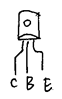
\includegraphics[width=0.1\linewidth]{figures/tri.png} % 数字表示放缩比例
  \caption{三极管外观图与管脚标注} % 图片标题
  \label{fig:Problem5} % 图片tag，用于交叉引用
\end{figure}

【数据分析】：hFE数值约为373说明三极管电流放大倍数约为373倍

\subsection{电源与万用表使用练习：}

\subsubsection{设定电源CH1、CH2电压分别为5V、12V，电流均为1A。用万用表直流电压档测量
实际输出电压并记录，计算电压偏差。}
% Table generated by Excel2LaTeX from sheet 'Sheet1'
\begin{table}[H]
  \centering
  \caption{实际输出电压与偏差}
    \begin{tabular}{|c|c|c|c|c|c|c|}
    \hline
    \multirow{2}[4]{*}{组别} & \multirow{2}[4]{*}{设定电源} & \multicolumn{4}{c|}{测量值} & \multirow{2}[4]{*}{实际误差} \bigstrut\\
\cline{3-6}          &       & 第1次   & 第2次   & 第3次   & 平均值   &  \bigstrut\\
    \hline
    1     & CH1（5V，1A） & 5.058V & 5.078V & 5.088V & 5.075V & 1.50\% \bigstrut\\
    \hline
    2     & CH2（12V，1A） & 12.074V & 12.061V & 12.085V & 12.073V & 0.61\% \bigstrut\\
    \hline
    \end{tabular}%
  \label{tab:addlabel}%
\end{table}%

\subsubsection{设定电源电压分别为正负5V，正负12V，用万用表直流电压档测量并记录。}
% Table generated by Excel2LaTeX from sheet 'Sheet1'
\begin{table}[htbp]
  \centering
  \caption{实际输出电压与偏差}
    \begin{tabular}{|c|c|c|c|c|c|c|}
    \hline
    \multirow{2}[4]{*}{组别} & \multirow{2}[4]{*}{设定电源} & \multicolumn{4}{c|}{测量值} & \multirow{2}[4]{*}{实际误差} \bigstrut\\
\cline{3-6}          &       & 第1次   & 第2次   & 第3次   & 平均值   &  \bigstrut\\
    \hline
    1     & ±5V   & 10.213V & 10.212V & 10.214V & 10.213V & 2.13\% \bigstrut\\
    \hline
    2     & ±12V  & 24.61V & 24.60V & 24.61V & 24.61V & 2.54\% \bigstrut\\
    \hline
    \end{tabular}%
  \label{tab:addlabel}%
\end{table}%

\subsubsection{设定电源CH1电压为1V，限定电流为0.5A，用万用表的“2A直流电流”档测量
短路限制电流并记录，计算设置偏差（电流测量时，将红表笔插到左边的2/20A输入孔，测
量结束恢复到电压/电阻测试位置）}

% Table generated by Excel2LaTeX from sheet 'Sheet1'
\begin{table}[H]
  \centering
  \caption{实际输出电流与偏差}
    \begin{tabular}{|c|c|c|c|c|c|}
    \hline
    \multirow{2}[4]{*}{设定电源} & \multicolumn{4}{c|}{测量值} & \multirow{2}[4]{*}{实际误差} \bigstrut\\
\cline{2-5}          & 第1次   & 第2次   & 第3次   & 平均值   &  \bigstrut\\
    \hline
    CH1（1V，0.5A） & 0.4821A & 0.4821A & 0.4820A & 0.4821A & -3.58\% \bigstrut\\
    \hline
    \end{tabular}%
  \label{tab:addlabel}%
\end{table}%

\subsubsection{思考}

【数据分析】：经多组设定电压和限定电流的测量，发现万用表测量电压和电流值与设定值相差不大，测量较精准。同时，在【电源与万用表使用练习】这整个实验中，output按下时电压电流可能会发生变化，可能是引起误差的原因


\subsection{信号源与示波器使用练习：}
\subsubsection{示波器探头接校准信号源，按傻瓜键“Autoset”，观察记录波形；使用光标法（按
示波器面板上的“Cursor”功能键）读取信号的幅度和周期（或频率）信息，并作相应记录。}
% Table generated by Excel2LaTeX from sheet 'Sheet1'
\begin{table}[htbp]
  \centering
  \caption{校准信号源的幅度与频率}
    \begin{tabular}{|c|c|}
    \hline
    幅度    & 频率 \bigstrut\\
    \hline
    2.03V & 1.000kHz \bigstrut\\
    \hline
    \end{tabular}%
  \label{tab:addlabel}%
\end{table}%

\begin{figure}[H]
  \centering
  \begin{minipage}[b]{0.4\linewidth}
      \centering
      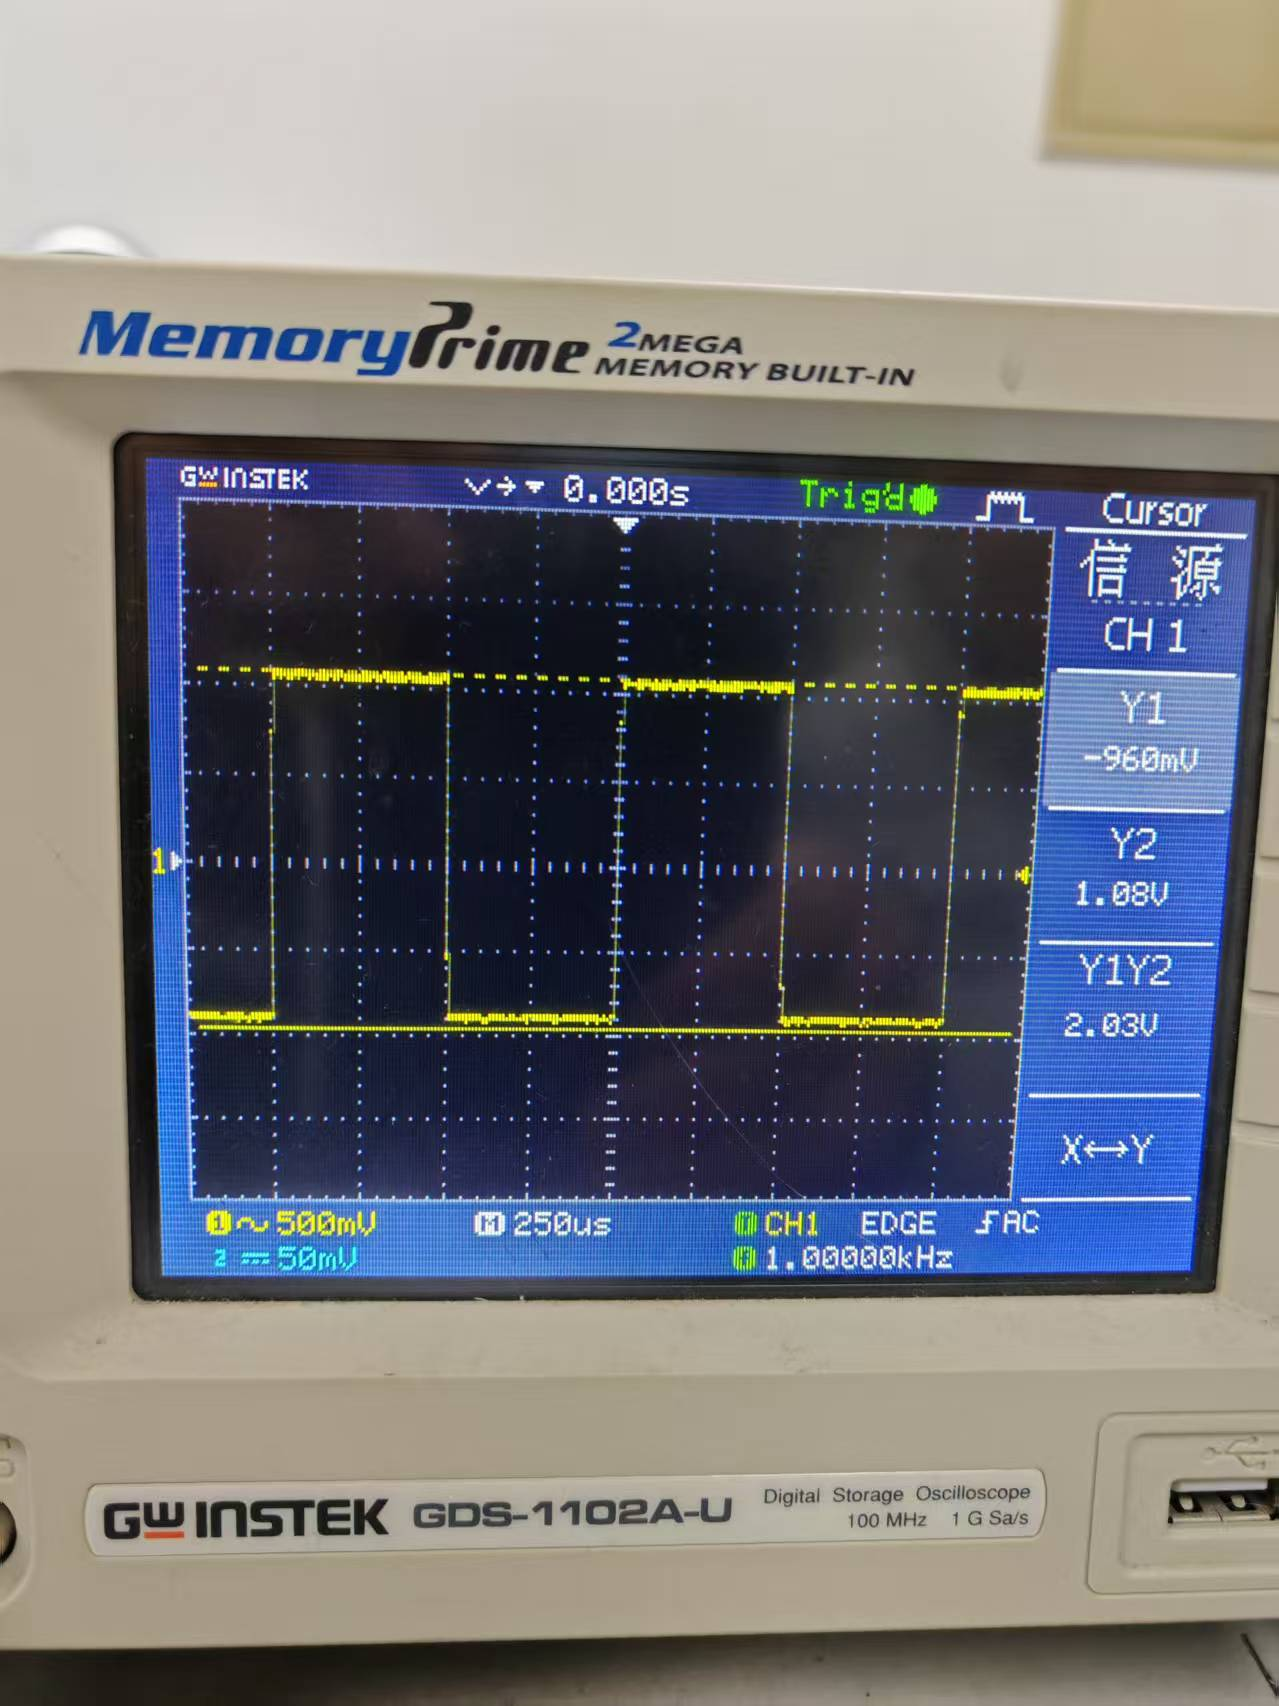
\includegraphics[width=0.9\textwidth]{figures/ex_v.jpg}
      \caption{校准信号源幅度测量图}
  \end{minipage}%
  \begin{minipage}[b]{0.4\linewidth}
      \centering
      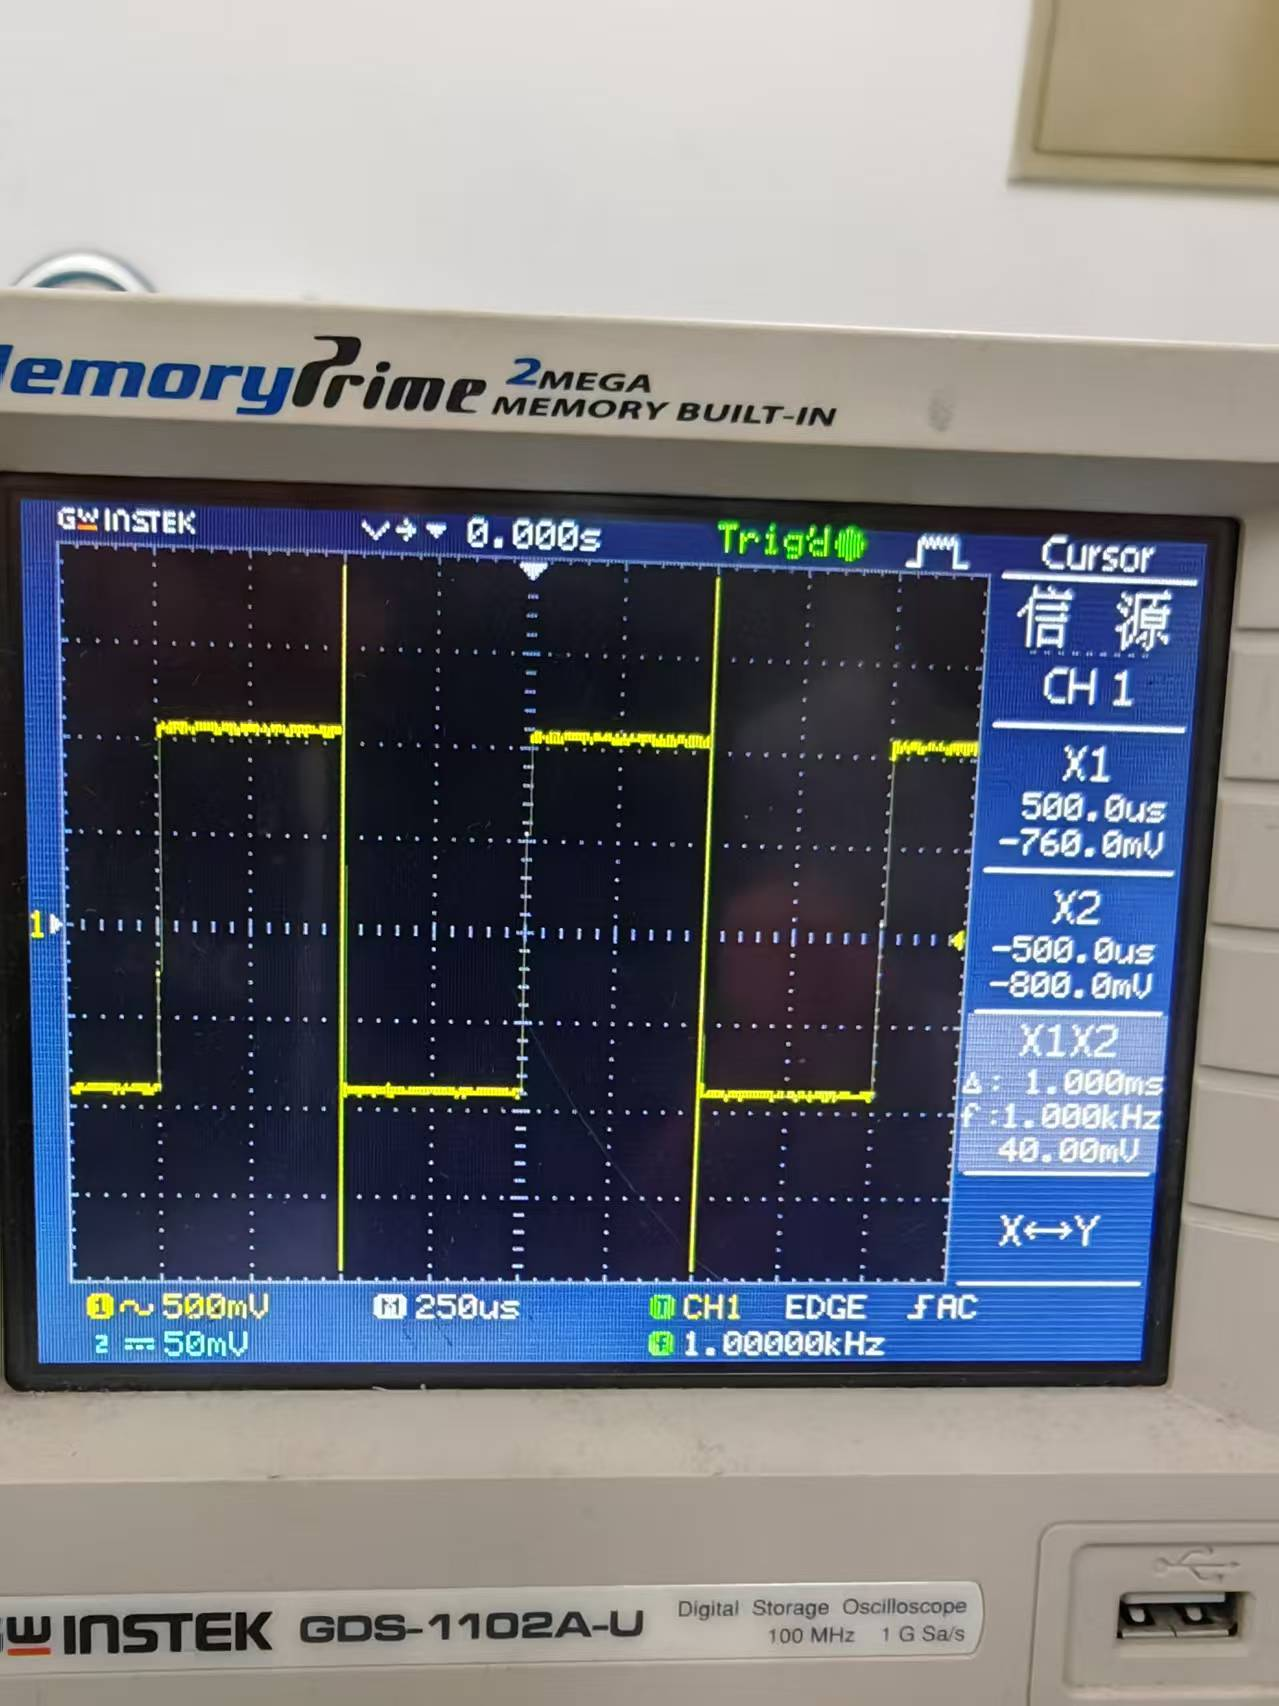
\includegraphics[width=0.9\textwidth]{figures/ex_f.jpg}
      \caption{校准信号源频率测量图}
  \end{minipage}
\end{figure}

\subsubsection{调节信号源，使信号源输出幅度为0.2Vp-p，频率分别为10KHz，100KHz，1MHz，
10MHz 的正弦波信号。用示波器CH1测量信号源的输出，选择触发通道为“CH1”，触发模式
为“自动”，调节触发电平“LEVEL”使得波形能稳定显示。调节相应的量程旋钮“VOLTS/DIV”，
和扫描周期旋钮“TIME/DIV”使得波形显示大小合适，记录设定的电压量程和扫描时间；按
测量键“Measure”，记录测量得到的波形的幅度和时间（或频率）参数。}
% Table generated by Excel2LaTeX from sheet 'Sheet1'
\begin{table}[H]
  \centering
  \caption{正弦波测量}
    \begin{tabular}{|c|c|c|c|c|}
    \hline
    设定频率  & 电压量程  & 扫描时间  & 测量幅度  & 测量频率 \bigstrut\\
    \hline
    10kHz & 50mV  & 25us  & 202mV & 9.960kHz \bigstrut\\
    \hline
    100kHz & 50mV  & 2.5us & 200mV & 100.4kHz \bigstrut\\
    \hline
    1MHz  & 50mV  & 250ns & 206mV & 1.009MHz \bigstrut\\
    \hline
    10MHz & 50mV  & 25ns  & 202mV & 10.15MHz \bigstrut\\
    \hline
    \end{tabular}%
  \label{tab:addlabel}%
\end{table}%

\begin{figure}[H]
  \centering
  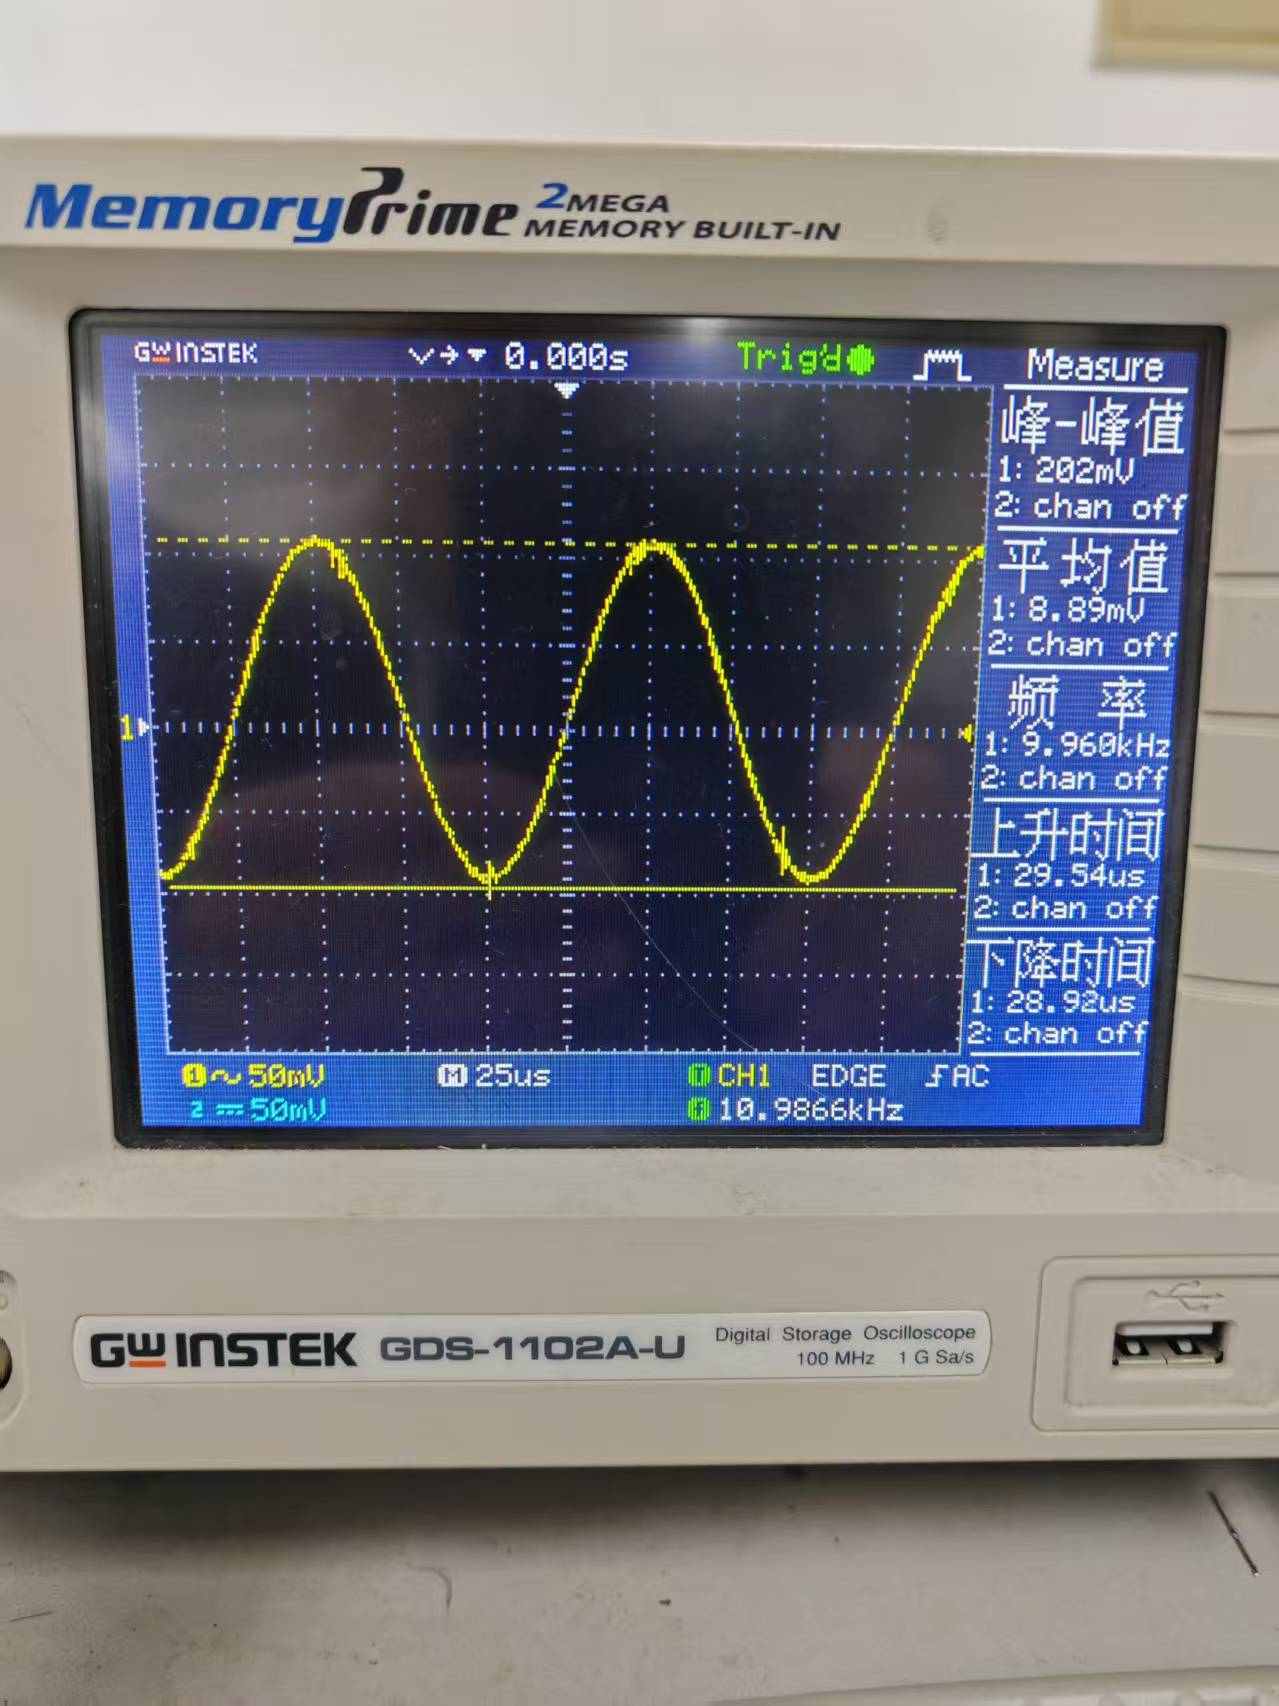
\includegraphics[width=0.5\linewidth]{figures/p2.jpg} % 数字表示放缩比例
  \caption{正弦波测量} % 图片标题
  \label{fig:Problem5} % 图片tag，用于交叉引用
\end{figure}


\subsubsection{在实验步骤（2）的基础上，改变信号波形：分别为方波、三角波，测量波形的幅
度和时间参数并记录。}

\begin{table}[H]
  \centering
  \caption{方波测量}
    \begin{tabular}{|c|c|c|c|c|}
    \hline
    设定频率  & 电压量程  & 扫描时间  & 测量幅度  & 测量频率 \bigstrut\\
    \hline
    10kHz & 50mV  & 25us  & 212mV & 10.00kHz \bigstrut\\
    \hline
    100kHz & 50mV  & 2.5us & 210mV & 100.1kHz \bigstrut\\
    \hline
    1MHz  & 50mV  & 250ns & 206mV & 999.8kHz \bigstrut\\
    \hline
    \end{tabular}%
  \label{tab:addlabel}%
\end{table}%

% Table generated by Excel2LaTeX from sheet 'Sheet1'
\begin{table}[H]
  \centering
  \caption{三角波测量}
    \begin{tabular}{|c|c|c|c|c|}
    \hline
    设定频率  & 电压量程  & 扫描时间  & 测量幅度  & 测量频率 \bigstrut\\
    \hline
    10kHz & 50mV  & 25us  & 218mV & 10.16kHz \bigstrut\\
    \hline
    100kHz & 50mV  & 2.5us & 196mV & 100.4kHz \bigstrut\\
    \hline
    500kHz & 50mV  & 500ns & 203mV & 501.2kHz \bigstrut\\
    \hline
    \end{tabular}%
  \label{tab:addlabel}%
\end{table}%

\begin{figure}[H]
  \centering
  \begin{minipage}[b]{0.4\linewidth}
      \centering
      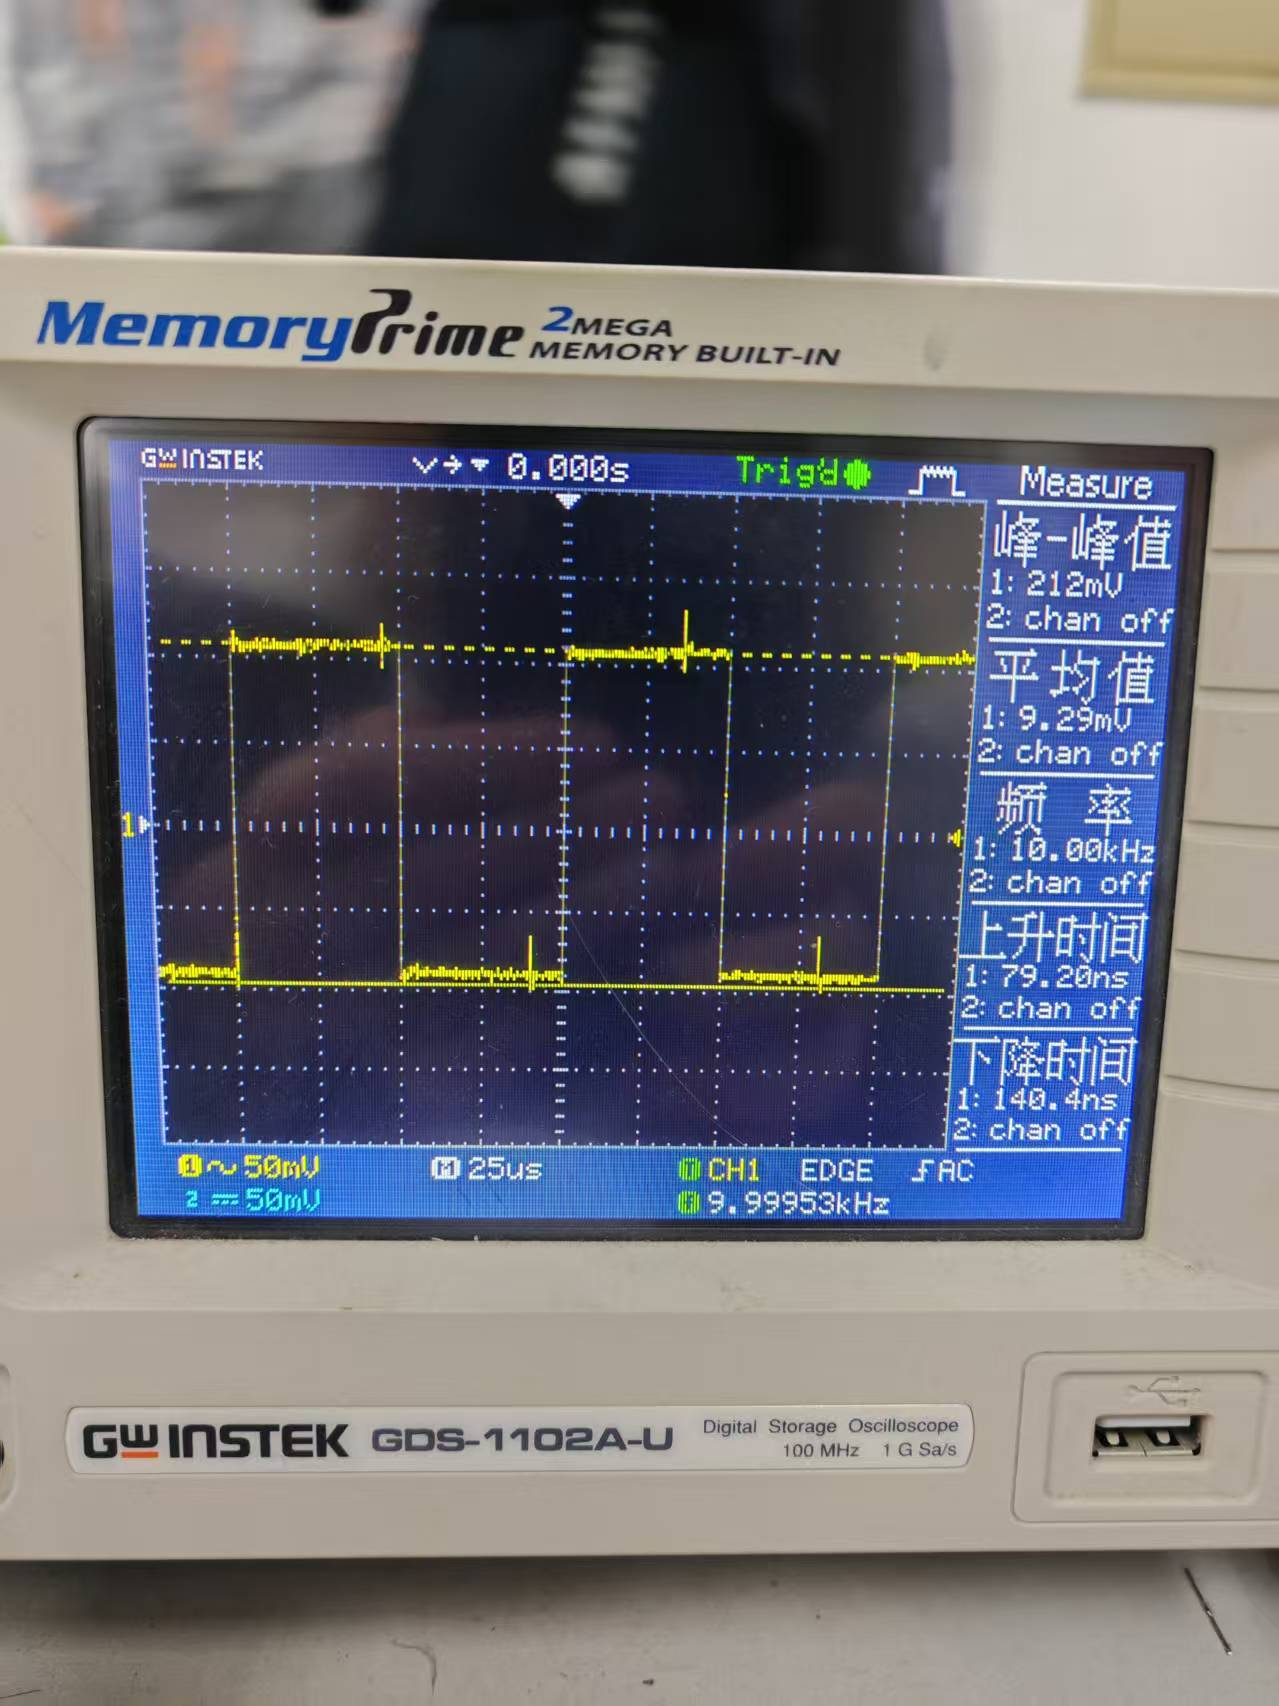
\includegraphics[width=0.9\textwidth]{figures/p1.jpg}
      \caption{方波测量}
  \end{minipage}%
  \begin{minipage}[b]{0.4\linewidth}
      \centering
      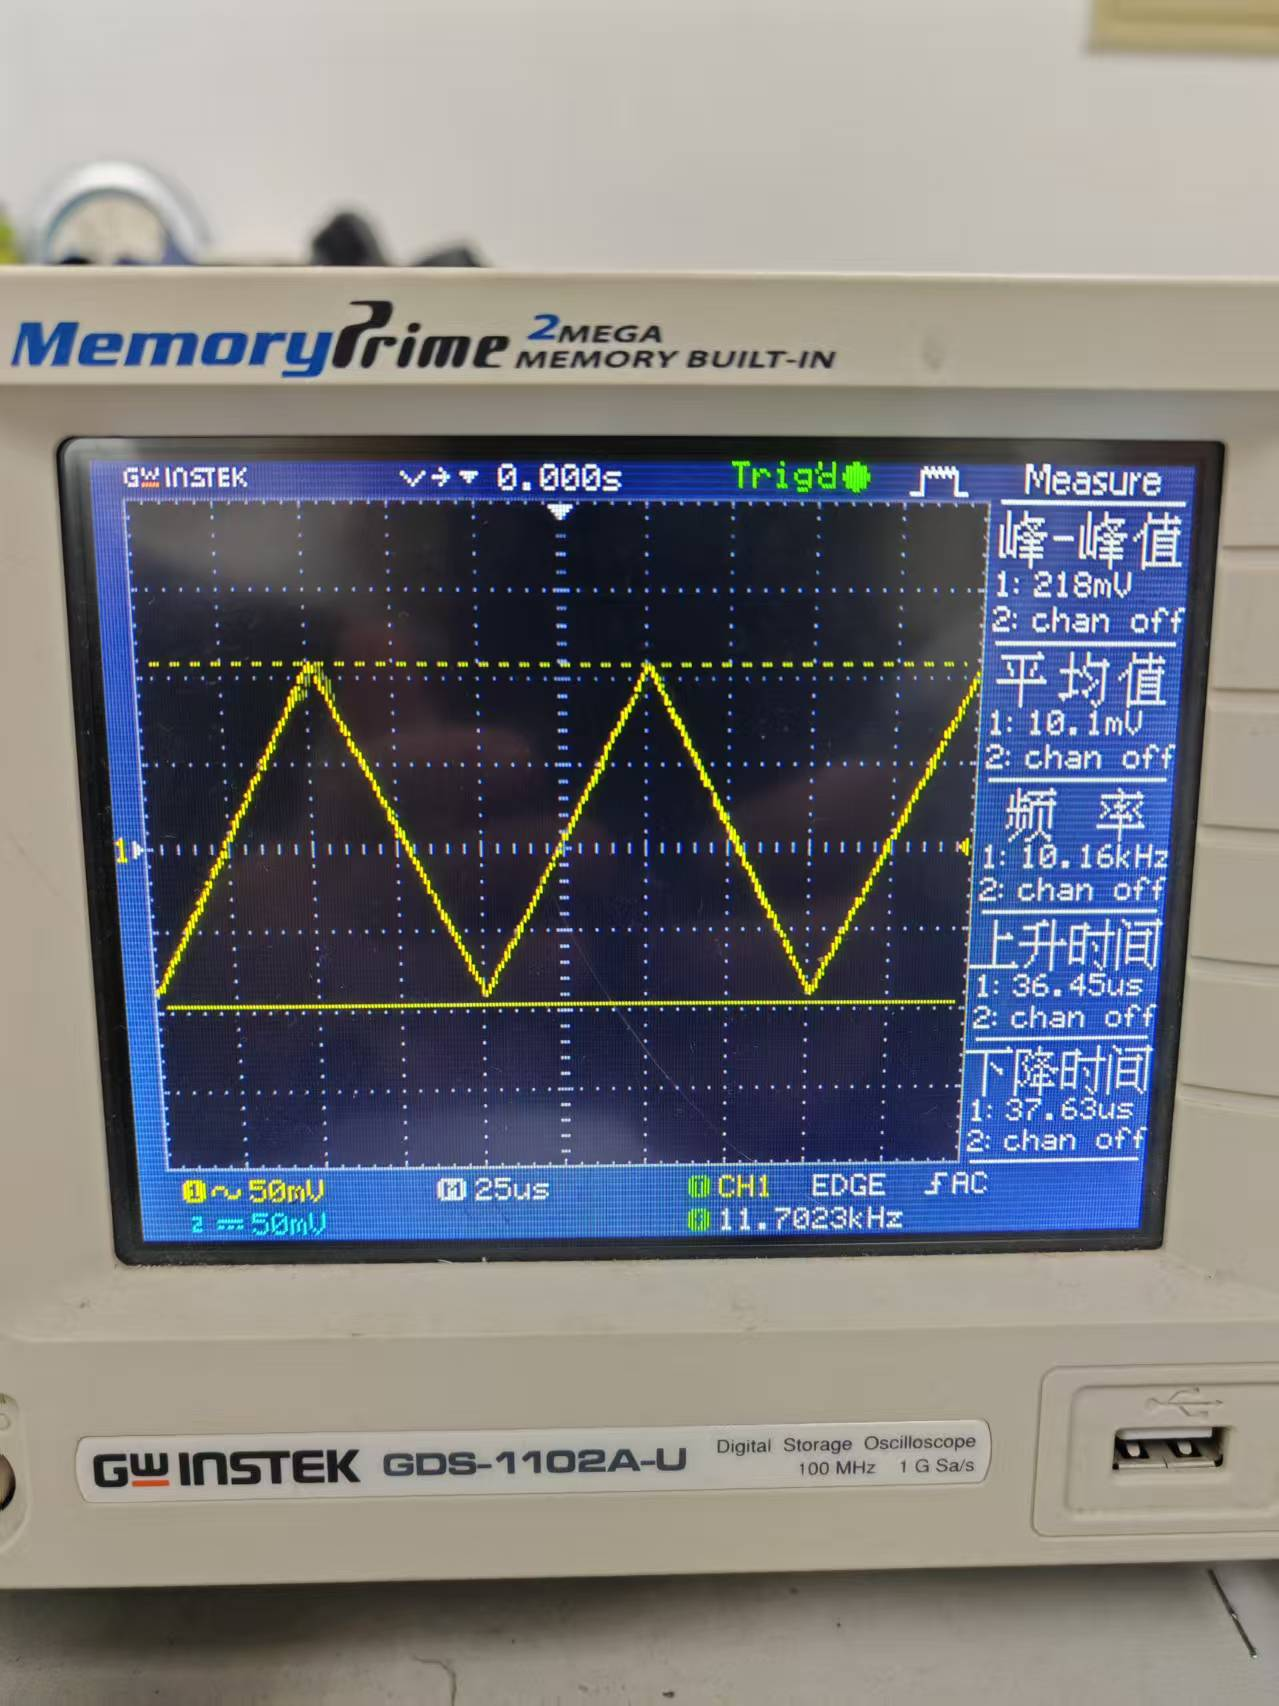
\includegraphics[width=0.9\textwidth]{figures/p3.jpg}
      \caption{三角波测量}
  \end{minipage}
\end{figure}

注：实验室方波频率上限为5MHz, 三角波频率上限为500kHz，故有些频率无法测量。

\subsubsection{信号源输出信号频率保持200KHz不变，在实验步骤（2）的基础上改变信号的幅
度，在0.5Vp-p与2Vp-p之间变化，步进0.5Vp-p用示波器观察信号的变化，采用光标法分
别测量幅度值并做相应的记录，分别计算测量偏差}

\begin{table}[H]
  \centering
  \caption{幅度测量}
    \begin{tabular}{|c|c|c|}
    \hline
    幅度    & 测量幅度  & 偏差 \bigstrut\\
    \hline
    0.5V  & 0.504V & 0.80\% \bigstrut\\
    \hline
    1.0V  & 0.998V & -0.20\% \bigstrut\\
    \hline
    1.5V  & 1.48V & -1.30\% \bigstrut\\
    \hline
    2.0V  & 2.04V & 2.00\% \bigstrut\\
    \hline
    \end{tabular}%
  \label{tab:addlabel}%
\end{table}%

\clearpage
\section{电路板波形测试数据及分析处理}
\subsection{呼吸灯调试}
\subsubsection{电源调整到12V，电流0.5A，连接电源线，打开电源的输出使能。}
\subsubsection{呼吸灯应该能正常工作，调整呼吸节奏到最快。}
\subsubsection{示波器测量集成电路1脚的波形，示波器采用直流耦合，采用STOP使波形停止（频
率太低时触发功能失效），光标法测量波形的幅度（Vp-p），周期。}
\subsubsection{示波器测量集成电路7脚的波形的幅度和周期。}
\subsubsection{1脚和7脚分别为何种波形？}
\subsubsection{调整电位器R3，观察波形周期的变化。}
% Table generated by Excel2LaTeX from sheet 'Sheet1'
\begin{table}[H]
  \centering
  \caption{集成电路1脚与7脚波形}
    \begin{tabular}{|c|c|c|c|}
    \hline
    引脚    & 幅度    & 周期    & 波形 \bigstrut\\
    \hline
    1脚    & 2.88V & 1.18s & 三角波 \bigstrut\\
    \hline
    7脚    & 9.35V & 1.17s & 方波 \bigstrut\\
    \hline
    \end{tabular}%
  \label{tab:addlabel}%
\end{table}%
\begin{figure}[H]
  \centering
  \begin{minipage}[b]{0.5\linewidth}
      \centering
      \includegraphics[width=0.9\textwidth]{figures/Phuxi2.jpg}
      \caption{集成电路1脚幅度}
  \end{minipage}%
  \begin{minipage}[b]{0.5\linewidth}
      \centering
      \includegraphics[width=0.9\textwidth]{figures/Phuxi1.jpg}
      \caption{集成电路1脚周期}
  \end{minipage}
\end{figure}
\begin{figure}[H]
  \centering
  \begin{minipage}[b]{0.5\linewidth}
      \centering
      \includegraphics[width=0.9\textwidth]{figures/Phuxi4.jpg}
      \caption{集成电路7脚幅度}
  \end{minipage}%
  \begin{minipage}[b]{0.5\linewidth}
      \centering
      \includegraphics[width=0.9\textwidth]{figures/Phuxi3.jpg}
      \caption{集成电路7脚周期}
  \end{minipage}
\end{figure}
调节电位器$R_3$,随着电阻的逐渐增大，呼吸灯呼吸频率逐渐降低，周期增长
\subsection{幸运转盘调试}
\subsubsection{电源调整到电压：5V，电流0.5A，连接电源线，打开电源的输出使能。}
\subsubsection{按一下启动键，幸运转盘应该能正常工作。}
\subsubsection{按住启动键，示波器测量集成电路U1的3脚波形，示波器采用直流耦合，光标法测量波形的幅度（Vp-p）、周期和负脉冲宽度。}
% Table generated by Excel2LaTeX from sheet 'Sheet1'
\begin{table}[htbp]
  \centering
  \caption{U1的3脚}
    \begin{tabular}{|c|c|c|c|}
    \hline
    \multirow{2}[4]{*}{U1的3脚波形} & 幅度    & 周期    & 负脉冲宽度 \bigstrut\\
\cline{2-4}          & 3.75V & 12.4ms & 88$\mu$s \bigstrut\\
    \hline
    \end{tabular}%
  \label{tab:addlabel}%
\end{table}%

\begin{figure}[H]
  \centering
  \begin{minipage}[b]{0.33\linewidth}
      \centering
      \includegraphics[width=0.9\textwidth]{figures/Pxingyun1.jpg}
      \caption{U1的3脚幅度$V_{p\_p}$}
  \end{minipage}%
  \begin{minipage}[b]{0.33\linewidth}
      \centering
      \includegraphics[width=0.9\textwidth]{figures/Pxingyun2.jpg}
      \caption{U1的3脚周期}
  \end{minipage}%
  \begin{minipage}[b]{0.33\linewidth}
      \centering
      \includegraphics[width=0.9\textwidth]{figures/Pxingyun3.jpg}
      \caption{U1的3脚负脉冲宽度}
  \end{minipage}
\end{figure}


\subsubsection{示波器测量集成电路U2的任何一个计数输出脚的波形，记录幅度、周期和正脉冲宽度，计算占空比。}
\begin{table}[H]
  \centering
  \caption{U2波形}
    \begin{tabular}{|c|c|c|c|c|}
    \hline
    \multirow{2}[4]{*}{U2} & 幅度    & 周期    & 正脉冲宽度 & 占空比 \bigstrut\\
\cline{2-5}          & 1.96V & 127ms & 12.8ms & 10.08\% \bigstrut\\
    \hline
    \end{tabular}%
  \label{tab:addlabel}%
\end{table}%


\begin{figure}[H]
  \centering
  \begin{minipage}[b]{0.33\linewidth}
      \centering
      \includegraphics[width=0.9\textwidth]{figures/Pxingyun5.jpg}
      \caption{U2的幅度$V_{p\_p}$}
  \end{minipage}%
  \begin{minipage}[b]{0.33\linewidth}
      \centering
      \includegraphics[width=0.9\textwidth]{figures/Pxingyun6.jpg}
      \caption{U2的周期}
  \end{minipage}%
  \begin{minipage}[b]{0.33\linewidth}
      \centering
      \includegraphics[width=0.9\textwidth]{figures/Pxingyun7.jpg}
      \caption{U2的正脉冲宽度}
  \end{minipage}
\end{figure}

\subsubsection{示波器测量三极管Q1发射极电压波形（采用直流耦合），按启动键，发射极电压升高，灯开始闪烁；松开启动键，电压开始下降，当灯刚好停止闪烁时，记录此时的发电极（E极）电压。}
% Table generated by Excel2LaTeX from sheet 'Sheet1'
\begin{table}[htbp]
  \centering
  \caption{三极管电压}
    \begin{tabular}{|c|c|}
    \hline
    \multirow{2}[4]{*}{三极管Q1发射极} & 停止闪烁时电压 \bigstrut\\
\cline{2-2}          & 3.12V \bigstrut\\
    \hline
    \end{tabular}%
  \label{tab:addlabel}%
\end{table}%

% Table generated by Excel2LaTeX from sheet 'Sheet1'

\subsection{贴片流水灯调试}
\subsubsection{连接电源+3V；}
\subsubsection{测试NE555的输出的信号（3脚）的幅度和频率；}
\subsubsection{测量上述信号的上升时间和下降时间；}
\begin{table}[htbp]
  \centering
  \caption{NE555输出信号}
    \begin{tabular}{|c|c|c|c|c|}
    \hline
    \multirow{2}[4]{*}{NE555} & 幅度    & 频率    & 上升时间  & 下降时间 \bigstrut\\
\cline{2-5}          & 2.42V & 13.02Hz & 110.0ns & 168.0ns \bigstrut\\
    \hline
    \end{tabular}%
  \label{tab:addlabel}%
\end{table}%


\begin{figure}[H]
  \centering
  \begin{minipage}[b]{0.5\linewidth}
      \centering
      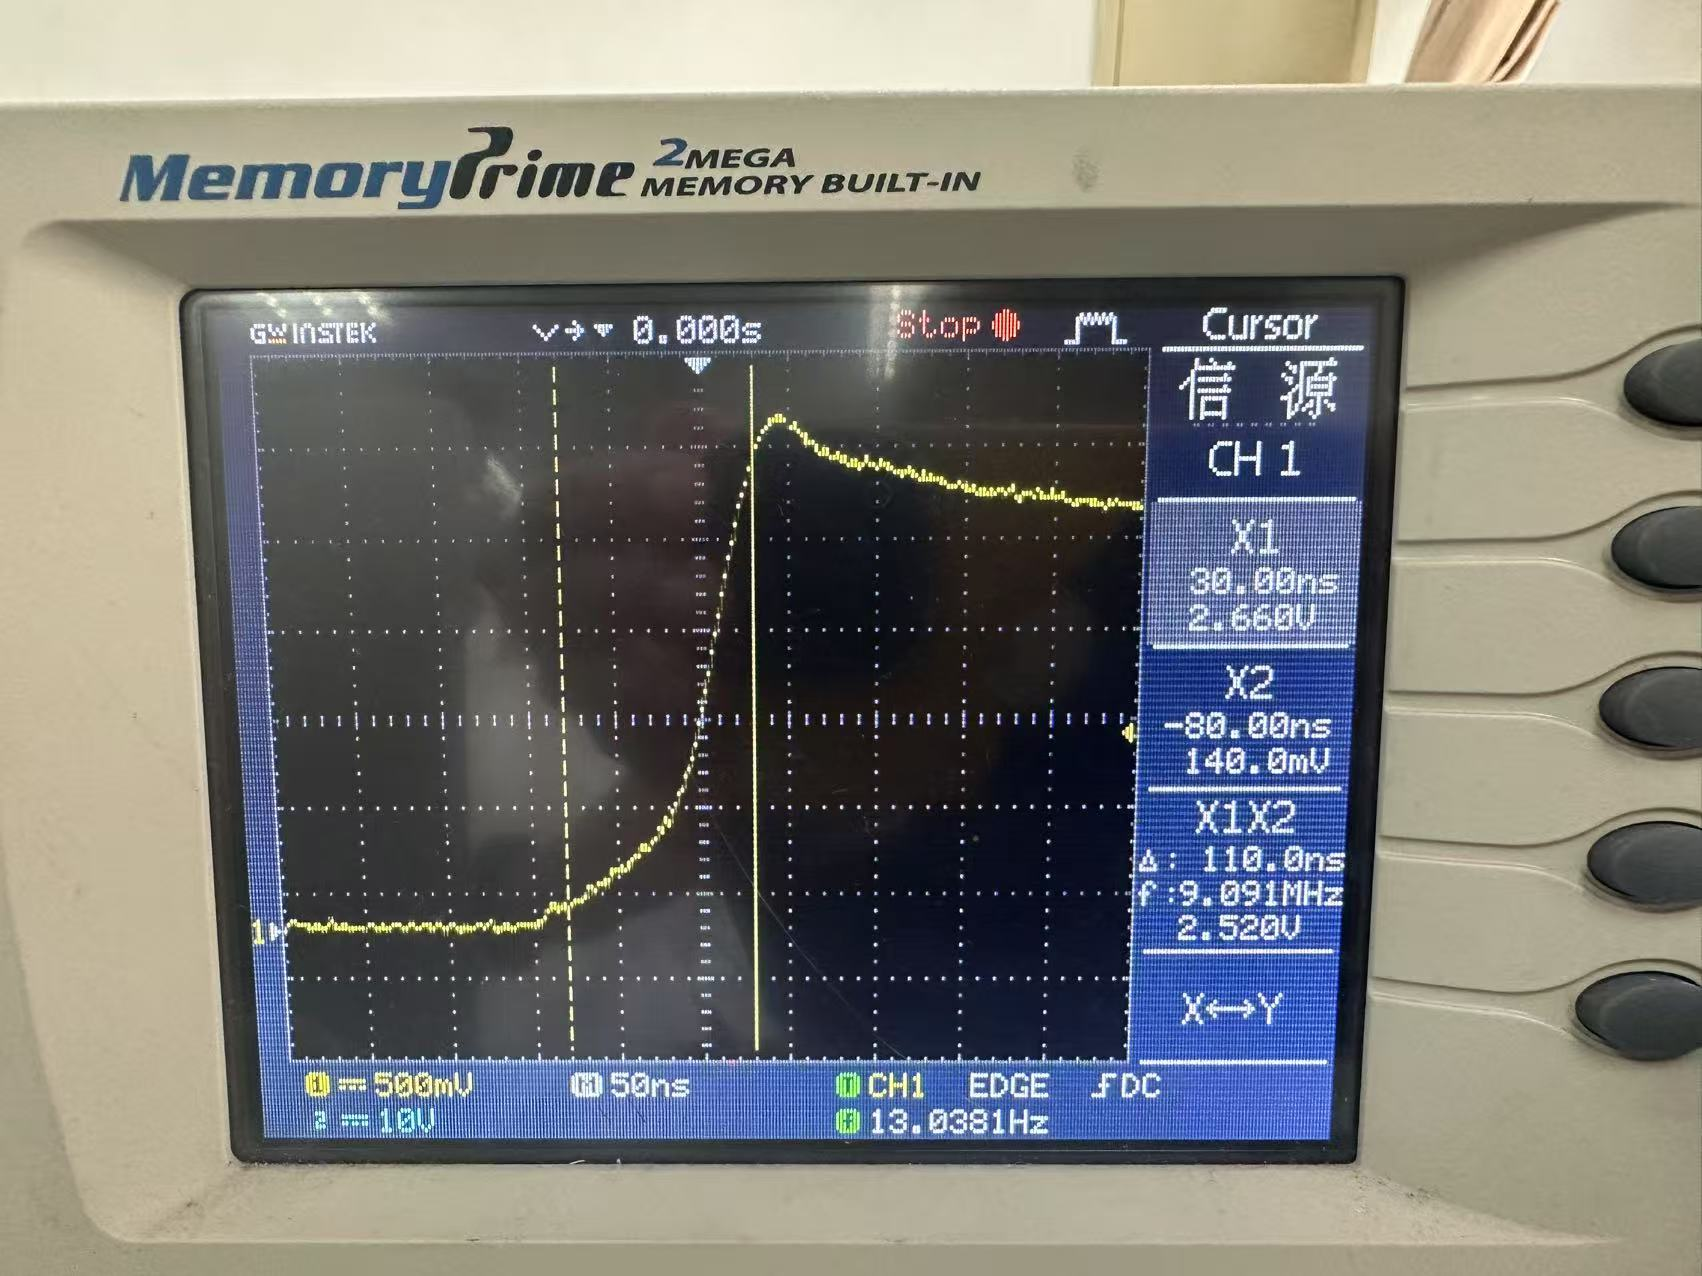
\includegraphics[width=0.9\textwidth]{figures/pliushui1.jpg}
      \caption{NE555上升时间}
  \end{minipage}%
  \begin{minipage}[b]{0.5\linewidth}
      \centering
      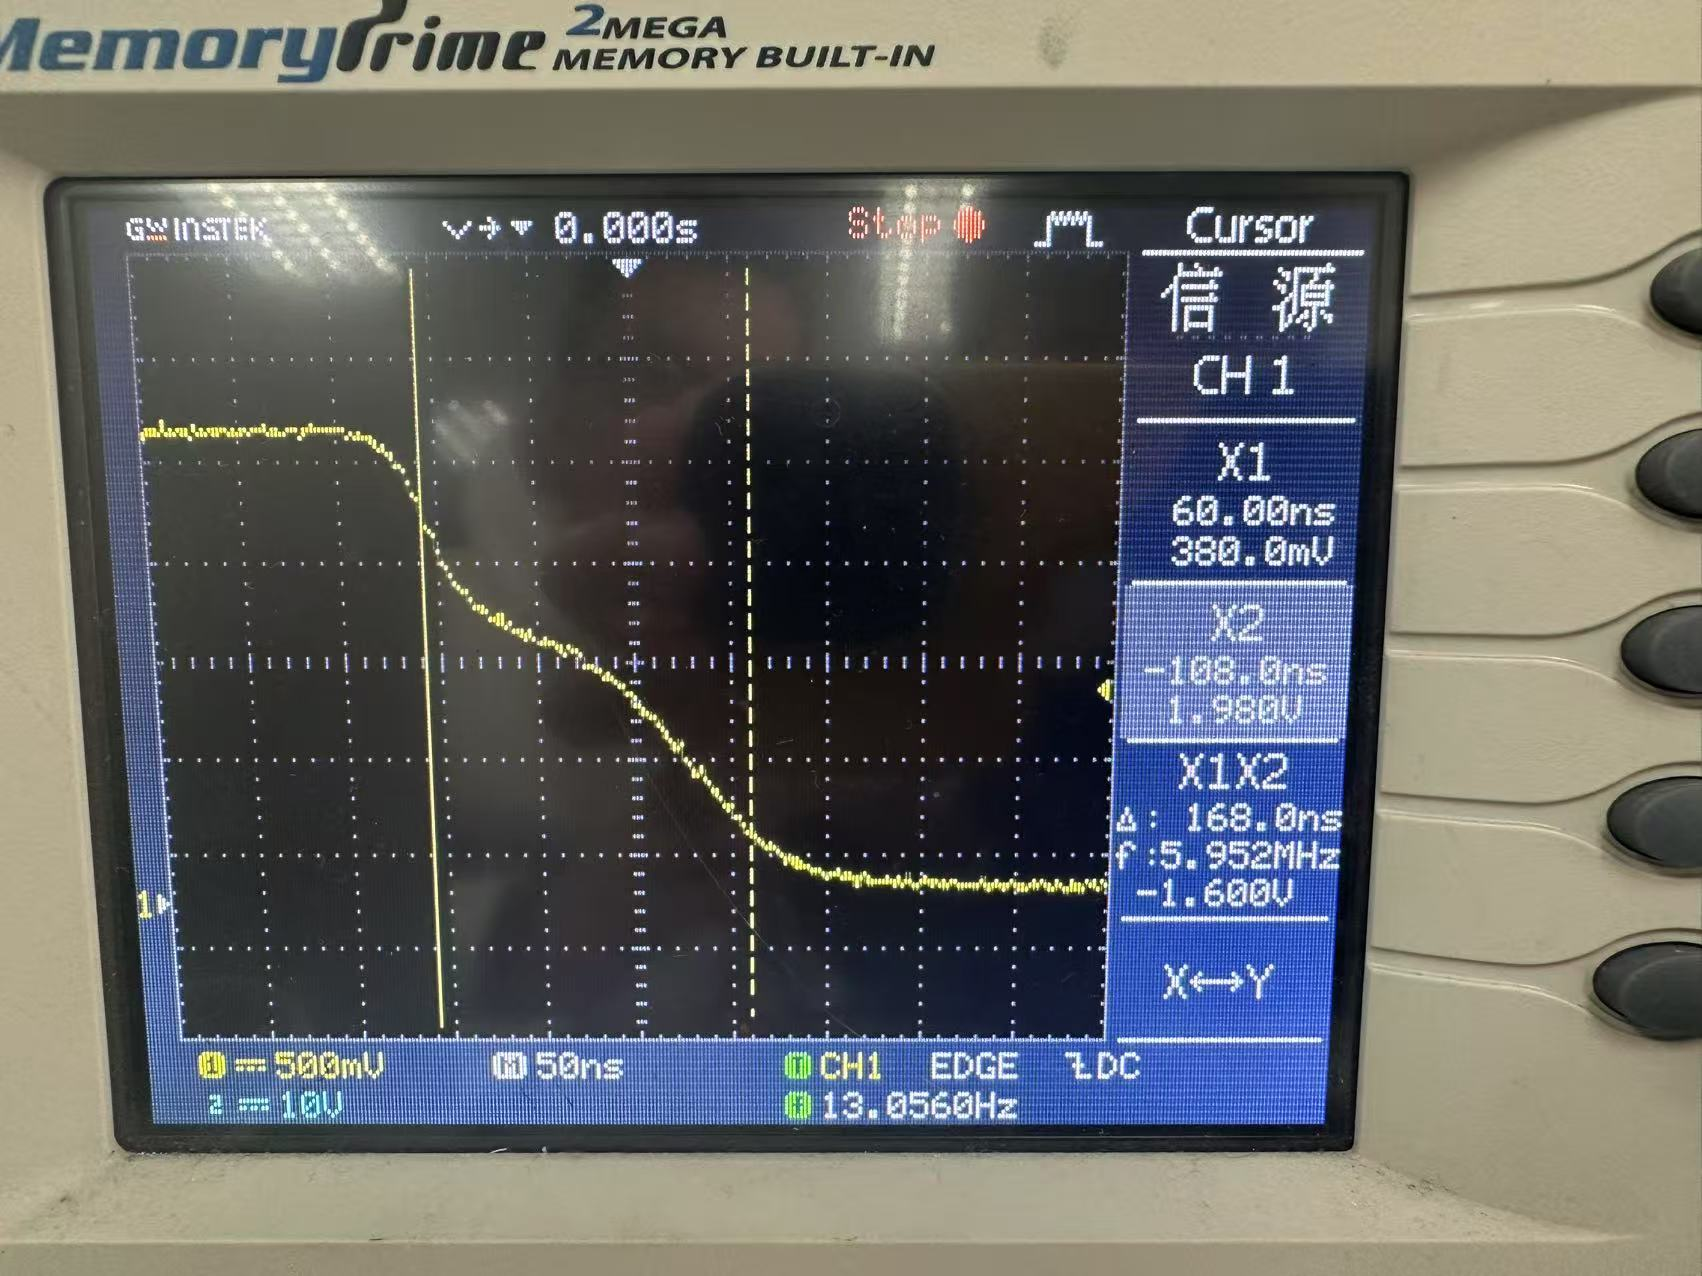
\includegraphics[width=0.9\textwidth]{figures/pliushui2.jpg}
      \caption{NE555下降时间}
  \end{minipage}
\end{figure}

\subsubsection{测试4017环形计数器输出波形的周期和脉冲宽度，计算信号的占空比，理论值应该是多少？}
% Table generated by Excel2LaTeX from sheet 'Sheet1'
\begin{table}[H]
  \centering
  \caption{4017 环形计数器输出波形}
    \begin{tabular}{|c|c|c|c|c|}
    \hline
    \multirow{2}[4]{*}{4017} & 周期    & 脉冲宽度  & 占空比计算值 & 占空比理论值 \bigstrut\\
\cline{2-5}          & 764ms & 76ms  & 10.14\% & 10\% \bigstrut\\
    \hline
    \end{tabular}%
  \label{tab:addlabel}%
\end{table}%

\begin{figure}[H]
  \centering
  \begin{minipage}[b]{0.5\linewidth}
      \centering
      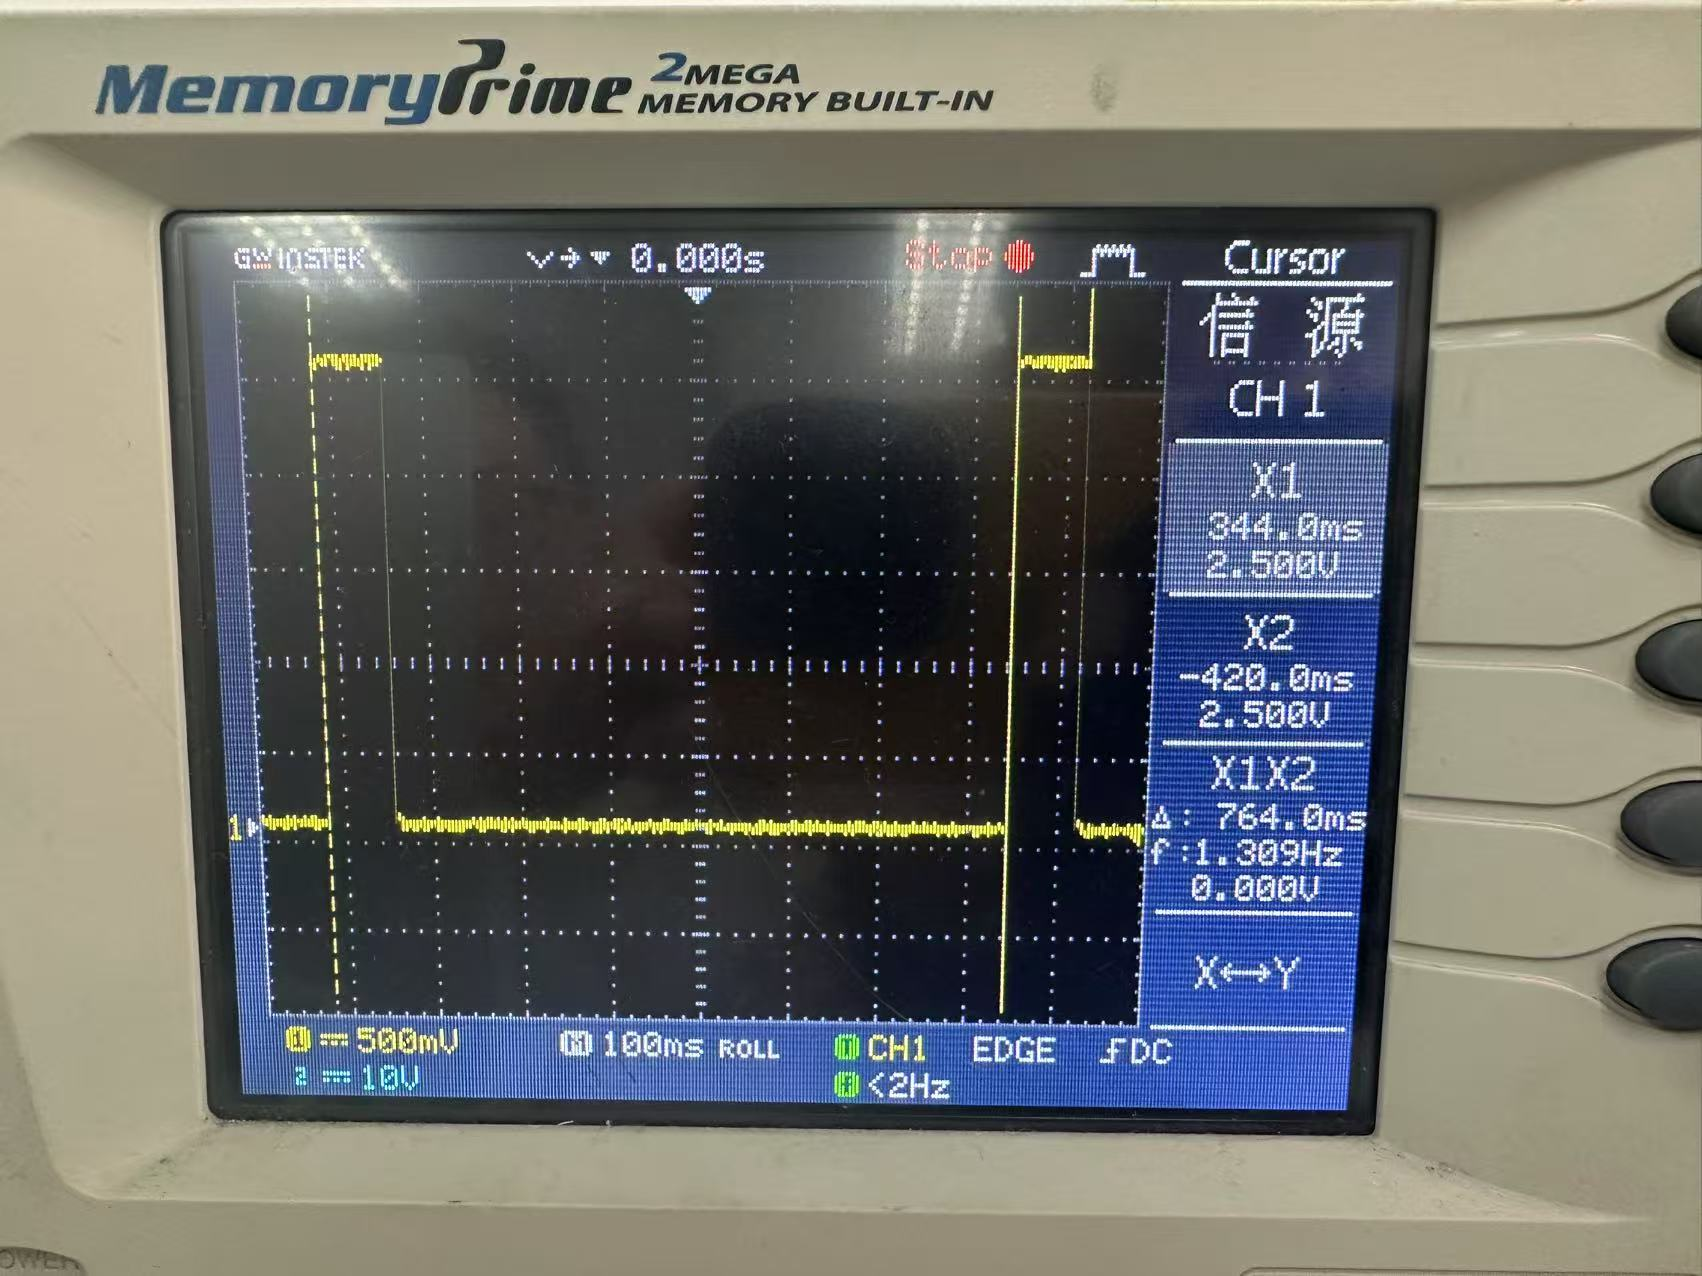
\includegraphics[width=0.9\textwidth]{figures/pliushui3.jpg}
      \caption{4017环形计数器输出波形周期}
  \end{minipage}%
  \begin{minipage}[b]{0.5\linewidth}
      \centering
      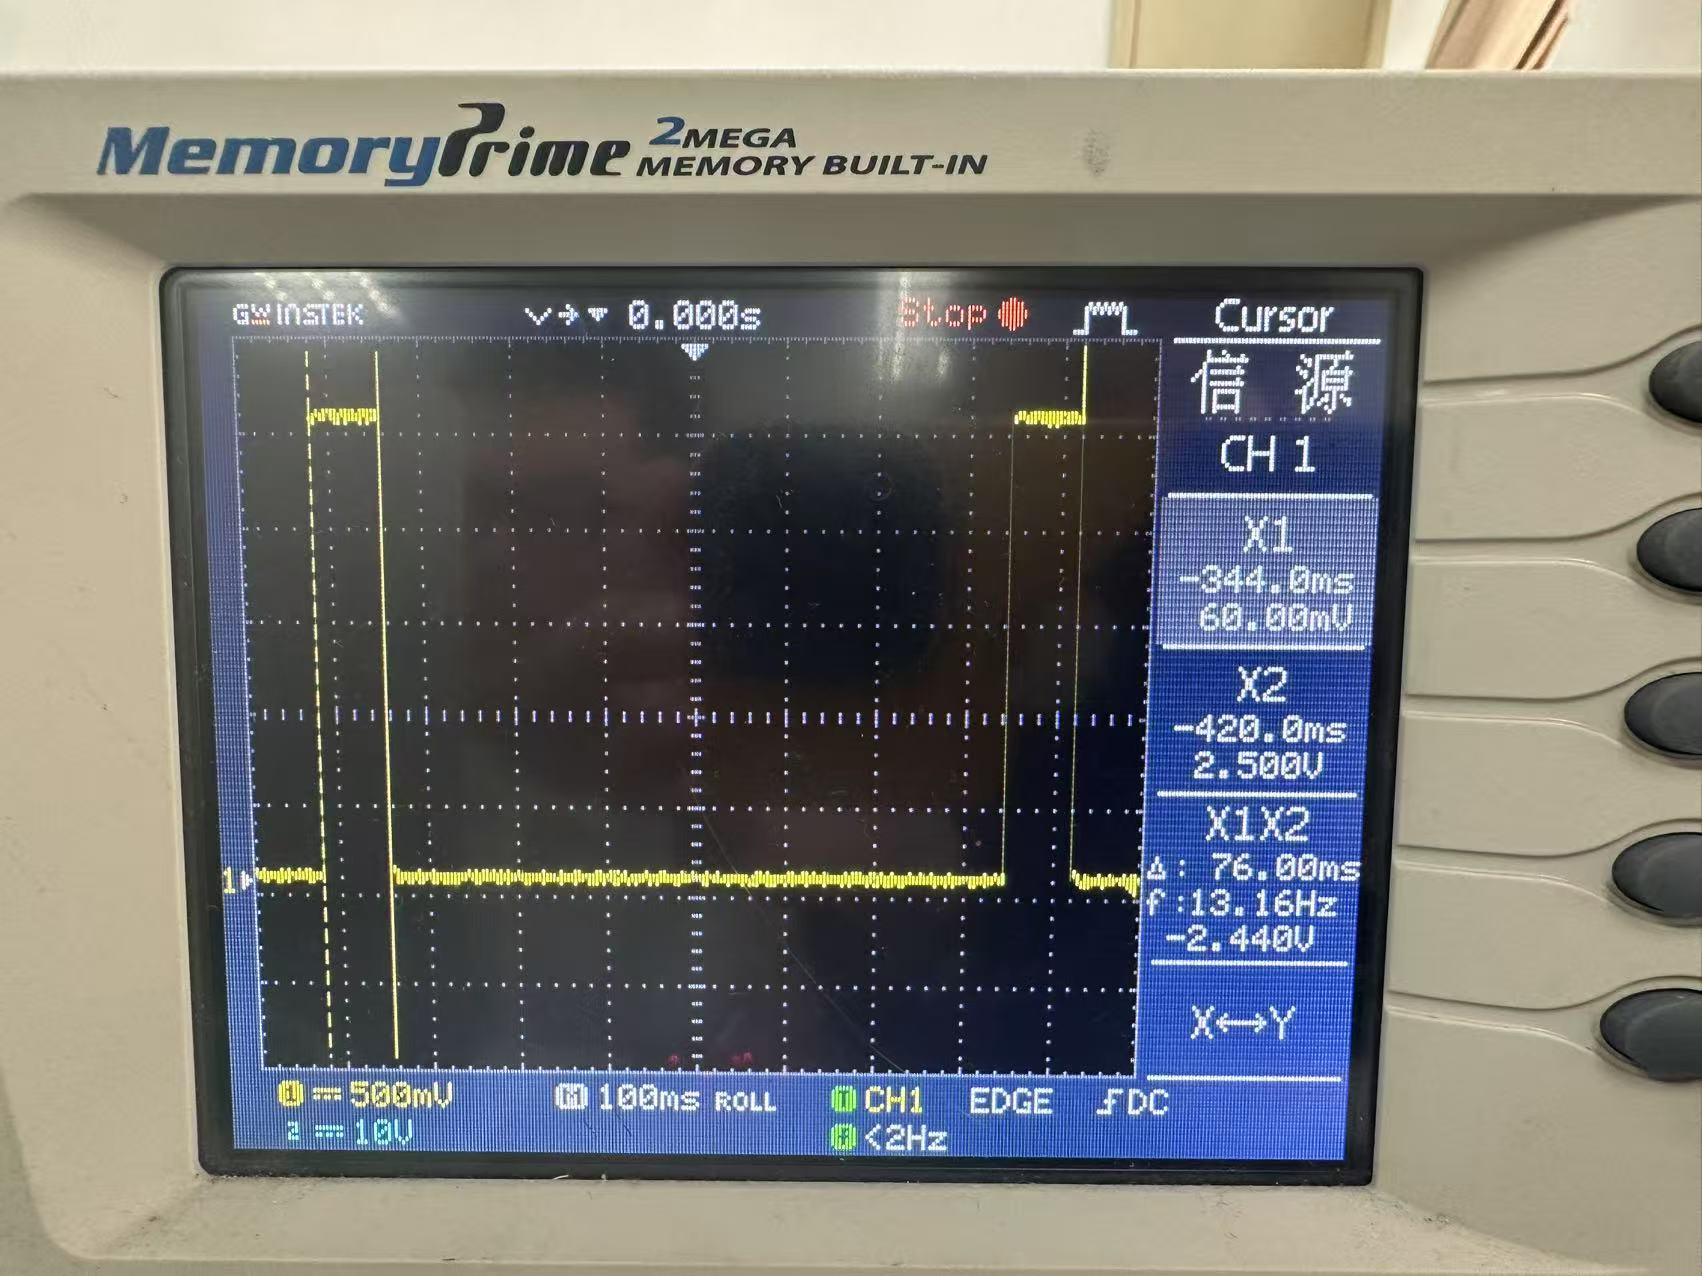
\includegraphics[width=0.9\textwidth]{figures/pliushui4.jpg}
      \caption{4017环形计数器输出波形脉冲宽度}
  \end{minipage}
\end{figure}
\subsubsection{测量Q1集电极信号周期。}
% Table generated by Excel2LaTeX from sheet 'Sheet1'
\begin{table}[H]
  \centering
  \caption{Q1集电极信号}
    \begin{tabular}{|c|c|}
    \hline
    Q1集电极周期 & 770ms \bigstrut\\
    \hline
    \end{tabular}%
  \label{tab:addlabel}%
\end{table}%

\begin{figure}[H]
  \centering
  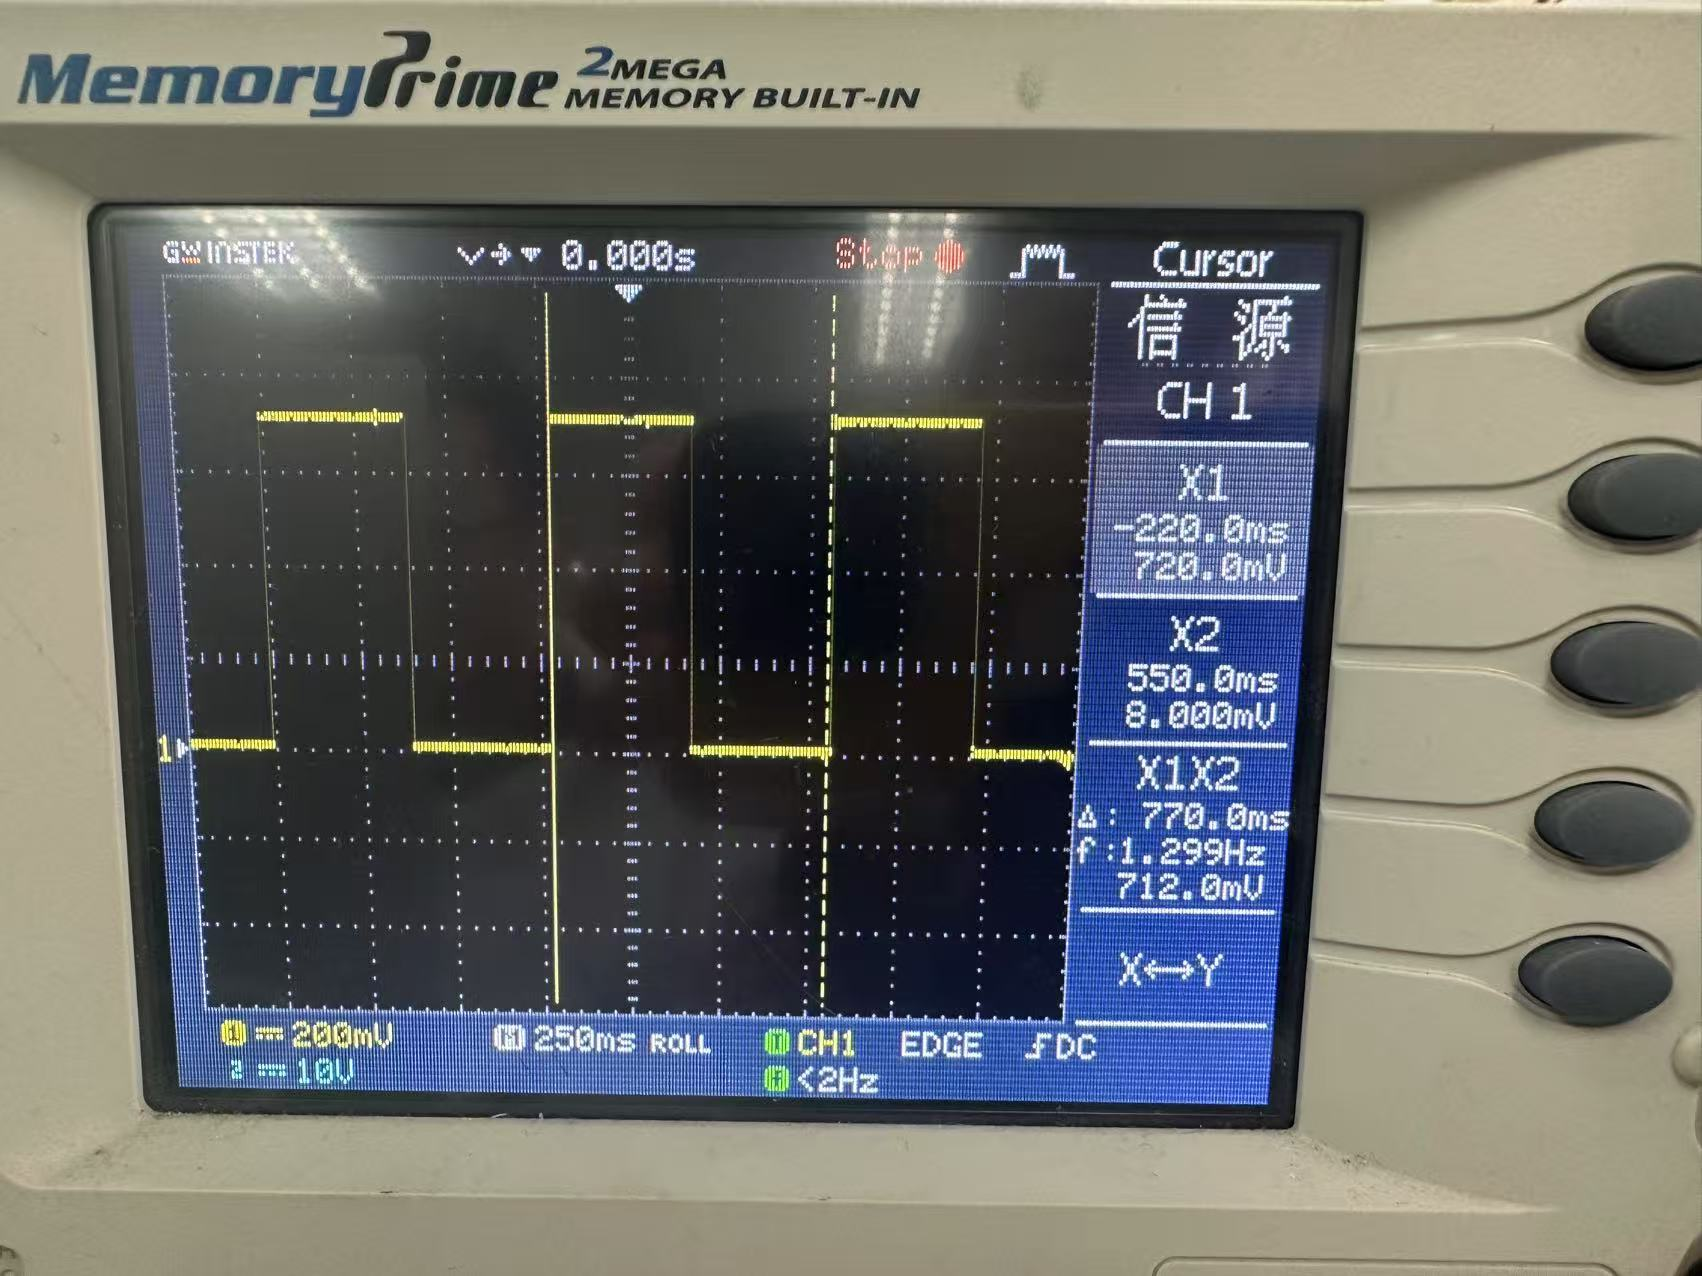
\includegraphics[width=0.5\linewidth]{figures/pliushui5.jpg} % 数字表示放缩比例
  \caption{Q1 集电极信号周期} % 图片标题
  \label{fig:Problem5} % 图片tag，用于交叉引用
\end{figure}

\section{实验总结}
\subsection{实验收获}
\begin{enumerate}
  \item 掌握了电子器件的相关知识，学会了如何识别电子器件。
  \item 了解了 PCB 的种类，手工焊接的步骤。
  \item 学会了双列直插器件与贴片器件的焊接。
  \item 学会了电源，万用表，示波器，信号发生器的使用。
  \item 学会如何使用仪器测试与调试电路
\end{enumerate}

\subsection{对课程内容、教学方法等的评价以及建议}

\begin{enumerate}
  \item 可以减少理论部分的讲解，增加实操部分的演示。
  \item 可以将实验讲解拆开，讲解一部分做一部分，并在后一部分对前一部分的疑惑进行解答
  \item 可以对教学 PPT 进行进一步的精简，让同学们更好的吸收消化。  
\end{enumerate}

\end{document}